\documentclass{article}
 
\usepackage{afterpage}
\usepackage{amsmath}
\usepackage[utf8]{inputenc}
\usepackage[sorting=none,block=ragged,style=numeric-comp]{biblatex}
\addbibresource{ref.bib}
\usepackage{fancyhdr}
\usepackage{float}
\usepackage{geometry}
 \geometry{
 a4paper
 }
\usepackage{graphicx}
\graphicspath{{images/}}
\usepackage{hyperref}
\usepackage{listings}
\usepackage[T1]{fontenc}
\usepackage{subcaption}
\usepackage{titlesec}
\usepackage{xcolor}

\newcommand{\angstrom}{\textup{\AA}}
\newcommand{\Cov}{\mathrm{Cov}}

\titleformat{\section}[display]
  {\normalfont\bfseries}{}{0pt}{\Large}

\title{Deep generative learning for next-generation drugs}
\author{Vadim \textsc{Bertrand}}
\date{}
\makeatletter
    \let\thetitle\@title
    \let\theauthor\@author
    \let\thedate\@date
\makeatother

\definecolor{dark}{RGB}{22,75,94}
\definecolor{lightgrey}{rgb}{.90,.90,.90}
\definecolor{codegreen}{rgb}{0,0.6,0}
\definecolor{codegray}{rgb}{0.5,0.5,0.5}
\definecolor{codepurple}{rgb}{0.58,0,0.82}
\definecolor{backcolour}{rgb}{0.95,0.95,0.92}
 
\lstdefinestyle{mystyle}{
    backgroundcolor=\color{backcolour},   
    commentstyle=\color{codegreen},
    keywordstyle=\color{magenta},
    numberstyle=\tiny\color{codegray},
    stringstyle=\color{codepurple},
    basicstyle=\footnotesize,
    breakatwhitespace=false,         
    breaklines=true,                 
    captionpos=b,                    
    keepspaces=true,                 
    numbers=left,                    
    numbersep=5pt,                  
    showspaces=false,                
    showstringspaces=false,
    showtabs=false,                  
    tabsize=2
}
\lstset{style=mystyle}

\hypersetup{
    colorlinks=true,
    linkcolor=black,
    filecolor=magenta,     
    urlcolor=blue,
    citecolor=blue,
}

\pagestyle{fancy}

\begin{document}
\newgeometry{
 top=20mm,
 bottom=20mm,
 left=20mm,
 right=20mm
}
\begin{titlepage}
	\begin{minipage}{0.5\textwidth}
		\begin{flushleft}
		    
\includegraphics[width=0.4\textwidth]{logo_ljk.png}
		\end{flushleft}
	\end{minipage}
	\begin{minipage}{0.5\textwidth}
        \begin{flushright}
            
\includegraphics[width=0.75\textwidth]{logo_im2ag.png}
		\end{flushright}
	\end{minipage}\\[1.5 cm]
	
    \begin{center}
        {\Large Université Grenoble Alpes - IM2AG\\[.5 cm]
        Master 1 Mathématiques et Applications, parcours Statistique et Science des Données (SSD)}\\[1.5 cm]
        
        \textsc{\LARGE Internship report}
        \\[.5 cm]
        \large realized at Laboratoire Jean Kuntzmann, Grenoble\\[.2 cm]
        May 9 - Sept. 2, 2022\\[1.5 cm]
	    
	    \rule{\linewidth}{0.2 mm} \\[1 cm]
	    {\huge \bfseries \thetitle}\\[.7 cm]
	    \rule{\linewidth}{0.2 mm} \\[1.5 cm]
    	
    	{\Large \theauthor}\\[1.5 cm]
    \end{center}
    
	\begin{minipage}{0.5\textwidth}
		\begin{flushleft} \large
		    \textbf{LJK supervisor}\\
		    Sergei \textsc{Grudinin}\\
		\end{flushleft}
	\end{minipage}
	\begin{minipage}{0.5\textwidth}
        \begin{flushright} \large
			\textbf{Academic supervisor} \\
			Adeline \textsc{Leclercq Samson}\\
		\end{flushright}
	\end{minipage}
\end{titlepage}
\restoregeometry
\pagebreak

\section*{Acknowledgments}

First of all, I would like to thank Adeline Leclercq Samson who coordinated and ensured the good proceedings of this internship. \\
Thank you again for reading this report and attending my defense, along side Marie Thieulin. \\

Then, I really enjoined sharing those few months with the other interns at IMAG, especially the few coming from SSD. I also wish all the best to Davy for his future thesis. \\
I am also grateful to Dima, who provided me good advice and insights on the work I conducted. Good luck in curing the world! \\

Finally, thanks a lot to Sergei Grudinin for his time, his availability and his patient supervision. It allows me to learn a lot in various fields during this highly enriching internship!

\newpage

\tableofcontents
\newpage

\section{Internship context}

I realized this internship as part of my first year of master's degree. As I was seeking both a stimulating subject and a benevolent environment, I chose to look for opportunities in research laboratories rather than companies. Research associate Sergei Grudinin welcomed me to the \textit{Données, Apprentissage et Optimisation} (DAO) team of \textit{Laboratoire Jean Kuntzmann} (LJK) in Grenoble. The research work conducted in the laboratory is at the boundary between mathematics and computer science, perpetuating Jean Kuntzmann's legacy. The DAO team focuses more precisely on optimization topics and their applications to machine learning, statistics and signal processing. \\
Sergei Grudinin's scientific interests include deep learning applied to structure and interaction of molecules in three dimensions (3D), such as protein-ligand interactions. This specific theme is at the heart of my internship on \textbf{Deep generative learning for next-generation drugs}. \\

But, what is a ligand? And, how is it related to proteins and drugs? \\
From antiquity, remedies were pretty much discovered by chance and recognized as such empirically. It is only during the 1970s that molecular approaches started to emerge. Those approaches rely on the establishment of a direct link between a pathology and an endogenous molecule, often a protein. Once this link is identified, molecular approaches are interested in finding an exogenous (small) molecule (the ligand) able to bind to the targeted protein and hopefully initiate an appropriate therapeutic response. \cite{WikiDrug} Therefore, here the ligand is the drug. \\
We refer to the couple formed by a protein and a bind-able ligand as the protein-ligand complex and to the protein's region where the ligand docks as the protein binding pocket. An illustration of such a complex is given in \textbf{Figure \ref{fig:complex}} below.
\begin{figure}[H]
    \centering
    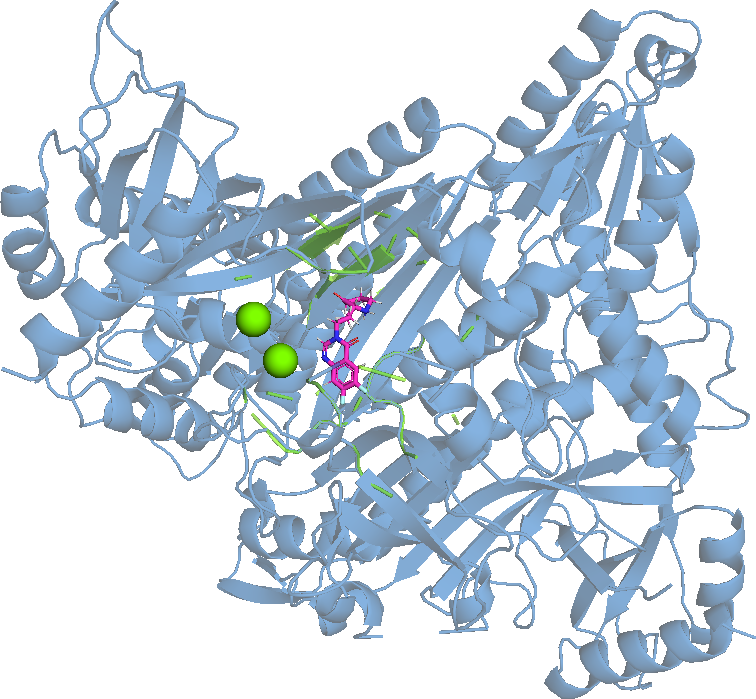
\includegraphics[height=6cm,width=\textwidth,keepaspectratio]{complex.png}
    \caption{2D visualization of a protein-ligand complex representation obtained using PyMOL \cite{PyMOL}. In blue the full protein, in green the protein pocket and in pink the ligand.}
    \label{fig:complex}
\end{figure}

\clearpage

\section{Problem statement}

\subsection{Modern drug design}

Drug discovery is nowadays vastly computer-aided. Finding an appropriate ligand given a protein might be theoretically realized by doing virtual screening against databases of small molecule candidates. However, current databases, such as ZINC20 \cite{zinc}, hold more than a billion ($10^9$) candidates, making exhaustive virtual screening unfeasible in practice. The best approaches can currently scan up to $10^6$ candidates, without accounting for the geometry and the specificity of the targeted protein.

\subsubsection{Neural networks to the rescue}

Over the past decade, machine learning and neural networks have allowed impressive progress in the Computer Vision and Natural Language Processing (NLP) domains. Those breakthroughs have already benefited several branches of life sciences, including biology. Since CASP14 \cite{CASP14}, thanks to DeepMind's AlphaFold \cite{AlphaFold}, the protein-folding problem (a protein's amino acid sequence should fully determine its 3D structure) as formulated by Chirstian Anfinsen in 1972 during his Nobel Prize acceptance speech, is considered to be solved. Closer to drug design, Convolutional Neural Networks (CNN) have been successfully used for protein-ligand interaction scoring \cite{PLscoringCNN}. Indeed, most structural bioinformatics problems can be addressed as NLP or 3D image processing tasks, with some additional constraints. A comprehensive review of the approaches proposed during CASP14 \cite{CASP14} has been proposed by Laine \textit{et al.} \cite{ProtRepr}.

\subsubsection{For protein-aware ligand generation}
\label{sec:pbstat}

In the scope of this internship we wanted to address a particularly ambitious problem: being given a protein, generating a bind-able ligand (the drug) in the binding pocket, without prior knowledge of exact geometrical conformation and chemical composition of the ligand. \\
This can be done by extending several different kinds of neural networks:
\begin{itemize}
    \item CNN \hyperref[sec:cnn]{[\S3.3.1]},
    \item Generative Adversarial Network (GAN),
    \item Graph Neural Network (GNN).
\end{itemize}
As it was hard to experiment all of them during the internship, we started with the most straightforward one, that is extension of CNN initaly designed for 2D image inpainting. 2D image inpainting is the process of reconstructing masked parts of an image. Those masked parts might correspond to corrupted or undesirable artifacts. The basic idea is to use the valid information around the mask to reconstruct it, using CNN. This topic is evolving quite fast and recent architectures have given impressive results, as shown in \textbf{Figure \ref{fig:2d_im_inp}}.
\begin{figure}[H]
    \begin{minipage}{0.5\textwidth}
    \centering
    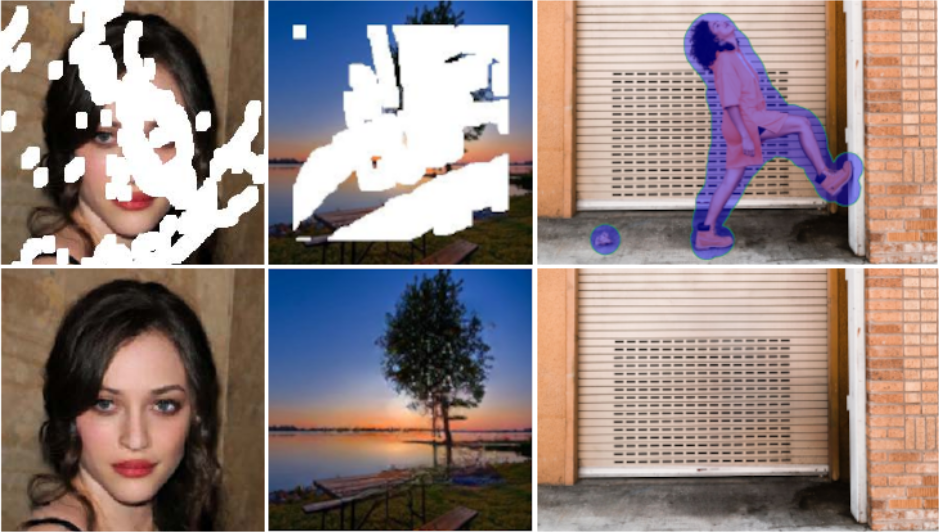
\includegraphics[height=3cm,width=\textwidth,keepaspectratio]{2d_im_inp.png}
    \end{minipage}
    \begin{minipage}{0.5\textwidth}
    \caption{Qualitative comparisons of 2D inpainting architectures. On the top are masked images, on the bottom are reconstructed ones. On the left is DSNet \cite{DSNet}, in the middle is RFR \cite{RFR}, on the right is LaMa \cite{LaMa}.}
    \label{fig:2d_im_inp}
    \end{minipage}
\end{figure}

\clearpage

\section{Proposed approach}

The neural network's kind and the data representation are strongly linked. I will therefore go into the particulars of the chosen complex's representation before detailing the employed architecture. But first, I need to present the dataset I have been using.

\subsection{The PDBbind database}
\label{sec:pdbbind}

I mentioned earlier some major progress realized in bioinformatics thanks to neural networks, but without underlying that they have been possible because of the prior knowledge of experimentally-solved structures of protein-ligand complexes. PDBbind \cite{PDBbind} is one of the databases allowing access to curated binding data. \\
In its 2020 version, PDBbind gathers 19,443 protein-ligand complexes in its "general set". This set includes a "refined set" of 5,316 complexes with better quality. Our dataset is composed of the "general set" with the exclusion of the "refined set", keeping this one for further validation. Thus, we are left with a bit more than 14,000 complexes. \\

For each complex in the database we are given files describing the full protein's structure, the protein's pocket structure and the associated ligand structure. Files regarding the protein are in Protein Data Bank format \cite{PDB} and the ligand's file is in a similar Structure Data File format. While those formats are found useful on many occasions, such as visualization with PyMOL for example, they are less practical for training and testing a neural network (or any machine learning model). \\
That is why the database was provided to me with an additional plain text file per complex. Those files contain the location of every protein's atom, plus the centroid and the orientation of every protein's amino acid residue. They also hold the location of every ligand's atom. In addition, atoms in those files were assigned a type. \\

\subsubsection{Building the final dataset}
\label{sec:dataset}

Although more handy and complete than the original ones, this file format was still a bit heavy to work with since it required parsing every file individually. That is why I decided to store all of them in an HDF5 file \cite{HDF5}. HDF5 and the associated Python library h5py \cite{h5py} let one store and manipulate large numerical data in a hierarchical fashion thanks to group, subgroup and dataset concepts. Access to groups, subgroups or datasets is done as if they were values of a hash map. Datasets are seen as numerical arrays. \\
After some refinements, I found the following structure easy to use:
\begin{itemize}
    \item complexes: top group holding one subgroup for each complex
    \begin{itemize}
        \item complex\_name: subgroups holding datasets
        \begin{itemize}
            \item atoms\_coordinates: $N_A \times 3$ array of coordinates
            \item atoms\_type: $N_A \times 1$ array of type
            \item protein\_atoms\_idx: $N_{Pa} \times 1$ array of protein's atoms' index
            \item ligand\_atoms\_idx: $N_{La} \times 1$ array of ligand's atoms' index
            \item residues\_frame\_origin: $N_R \times 3$ array of residues' origin
            \item residues\_frame\_axes: $N_R \times 3 \times 3$ array of residues' orientation axes
        \end{itemize}
        \item ...
    \end{itemize}
\end{itemize}

I randomly divided the dataset into a training set and a test set with sizes of respectively 80\% and 20\% of the full dataset, giving about 11,000 and 3,000 complexes in each of them. Again, the HDF5 format proved to be quite convenient as it allows attributes (such as names of the complexes in the training or the test sets) to be attached to groups, subgroups or datasets.

\subsubsection{"Hard" splitting of the dataset}
\label{sec:hard}

Creating training and test sets randomly from a sufficiently large dataset allows both diversity inside the sets and some similarity between them. It is desirable in most use-cases when the new data used for prediction is well represented by the sets employed for training and testing. \\
However, given the huge diversity in all the existing proteins, it is very likely that a protein for which biologists are interested in finding a bind-able ligand will be poorly represented by our limited dataset. Therefore, we would like our network to learn the interactions between atoms (because those do not change from one protein to the other) and generate ligands' atoms from that learning instead of generating a ligand based on the full structure of a protein. To validate this behaviour we decided to create an "hard" test set composed of the proteins least similar to the others.

\paragraph{Similarity between proteins}
Proteins can be expressed as strings using their amino acid sequence. The Levenshtein distance can then be used to compute the minimum number of single-character edits (either insertion, deletion or substitution) required for two strings to match. Its recursive implementation can be formulated as:
$$
lev(a, b) = \left\{
    \begin{array}{ll}
        \vert a \vert & \mbox{if } \vert b \vert = 0 \\
        \vert b \vert & \mbox{if } \vert a \vert = 0 \\
        lev(tail(a), tail(b)) & \mbox{if } a[0] = b[0] \\
        1 + min \left\{
            \begin{array}{ll}
                lev(tail(a), b) \\
                lev(a, tail(b)) \\
                lev(tail(a), tail(b))
            \end{array}
        \right. & \mbox{otherwise}
    \end{array}
\right.
$$
where \textit{tail} returns all the characters of a string, except for the first one. \\
Actual implementations of the Levenshtein distance (such as the Wagner-Fisher algorithm \cite{WFal}) use dynamic programming to avoid computing several times the distances between the same substrings and make the implementation usable in practice (while still having a time and space complexity of $\mathcal{O}(nm)$). \\

Amino acid sequences can be of very unequal lengths, leading to large distances even though the smaller sequence might be very close to a subpart of the longer one. To address this undesirable behaviour, it is common to compute the distance for all the possible alignments of the shorter sequence in the longer sequence and use the smallest one: 
$$
lev\_partial(a, b) = \left\{
    \begin{array}{ll}
        lev(a, b) & \mbox{if } \vert a \vert = \vert b \vert \\
        \min_{s \subset a, \vert s \vert >= \vert b \vert}lev(s, b) & \mbox{if } \vert a \vert > \vert b \vert \\
        \min_{s \subset b, \vert s \vert >= \vert a \vert}lev(a, s) & \mbox{if } \vert a \vert < \vert b \vert
    \end{array}
\right.
$$
Since the time complexity is now $\mathcal{O}(n^2m)$, implementations often do not provide an optimal solution for long sequences in order to keep it usable in practice. \\

The normalized similarity (ranging in [0, 1]) can finally be obtain using the following formula:
$$
sim(a, b) = 1 - lev\_partial(a, b) / max(\vert a \vert, \vert b \vert)
$$

I successfully used the Python \cite{Python} library RapidFuzz \cite{RapidFuzz} to compute in a very reasonable time (less than an hour with a desktop computer) the pairwise similarities (around 100 million) of the about 14,000 proteins in our dataset.

\paragraph{Splitting}
The splitting should satisfy two criteria:
\begin{itemize}
    \item the training and test set sizes are equal to 80\% and 20\% of the full dataset's size, respectively,
    \item the elements of the test set are least similar to those in the training set.
\end{itemize}
The following brute-force approach leads to such a splitting:
\begin{lstlisting}
import numpy as np

def brute_force(similarities: np.ndarray, proteins_name: np.ndarray, train_proportion: float):
    n_test = int(len(proteins_name) * (1 - train_proportion))
    test_set = []
    for _ in range(n_test):
        sum_similarities = similarities.sum(axis=0)
        idx = np.argmin(sum_similarities)
        test_set.append(proteins_name[idx])
        similarities = np.delete(np.delete(similarities, idx, axis=1), idx, axis=0)
        proteins_name = np.delete(proteins_name, idx)
    return proteins_name, test_set
\end{lstlisting}
The sequence with the smallest summed similarities is added to the test set and removed from the similarity matrix. The process is repeated until the test set is filled with the required number of proteins. This implementation is highly inefficient since the summed similarities are sorted at each iteration. It could be slightly approximated while greatly improving its complexity by sorting the summed similarities only once and retrieving the $n_{test}$ proteins with the smallest summed similarities:
\begin{lstlisting}
import numpy as np

def approx(similarities: np.ndarray, proteins_name: np.ndarray, train_proportion: float):
    n_test = int(len(proteins_name) * (1 - train_proportion))
    sum_similarities = similarities.sum(axis=0)
    less_similar = np.argsort(sum_similarities)[:n_test]
    test_set = proteins_name[less_similar]
    mask = np.ones(len(proteins_name), dtype=bool)
    mask[less_similar] = False
    return proteins_name[mask], test_set
\end{lstlisting}
As we can see in \textbf{Figure \ref{fig:splitting}}, the two variants give very close test sets distributions and the test set is indeed formed with the most dissimilar proteins.
\begin{figure}[H]
    \centering
    \begin{subfigure}{.5\textwidth}
        \centering
        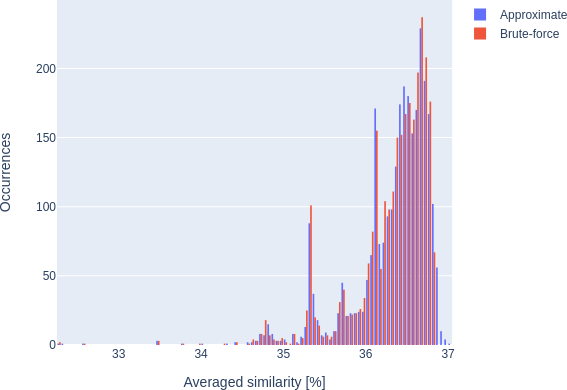
\includegraphics[height=6cm,width=\textwidth,keepaspectratio]{splitting_test_sets.png}
        \caption{Averaged similarities of the test sets' proteins.}
        \label{fig:splitting_test_sets}
    \end{subfigure}%
    \begin{subfigure}{.5\textwidth}
        \centering
        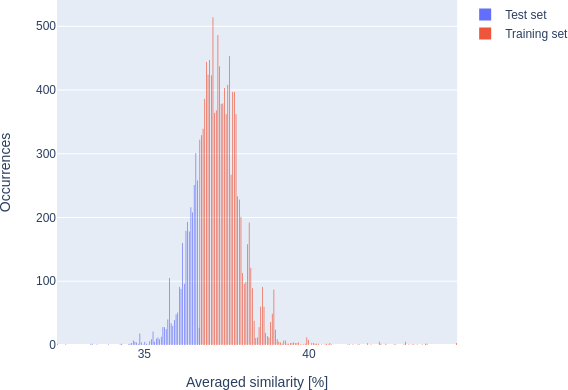
\includegraphics[height=6cm,width=\textwidth,keepaspectratio]{splitting_sets.png}
        \caption{Averaged similarities with approximate splitting.}
        \label{fig:splitting_sets}
    \end{subfigure}
    \caption{Histograms of the averaged similarities between every protein and the others.}
    \label{fig:splitting}
\end{figure}

\subsection{Representing the protein-ligand complex}

Since our neural network will be based on 2D image inpainting architectures, we want a representation of the protein-ligand complex close enough to an image, while embedding information specific to biological objects. \\

Of course, the periodic table's typisation of the atoms forming a molecule (and a protein) is an important characteristic. But it is not enough to describe the interactions taking place at the atomic level. That is why, as mentioned earlier, we employ another typisation, adding to the periodic table crucial information regarding the atom's bounds. There were in total 167 and 40 different new atom types for proteins and ligands, respectively.

\subsubsection{From the amino acid residues representation}

As shown in \textbf{Figure \ref{fig:in_equi_variance}}, it is often important when building a neural network to ensure that it is invariant or equivariant to translation and/or rotation. \\
\begin{figure}[H]
    \centering
    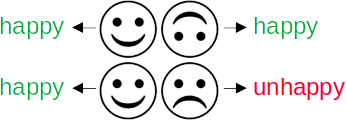
\includegraphics[height=3cm,width=\textwidth,keepaspectratio]{in_equi_variance.png}
    \caption{Illustration of the concepts of invariance and equivariance. Top row: a network should be \textit{invariant} to a rotation of the full face. Bottom row: but it should be \textit{equivariant} to a rotation of only the mouth.}
    \label{fig:in_equi_variance}
\end{figure}
In order to approach the representation of an image and preserve \textit{invariance} to rotation of an input protein, I built a $24 \times 24 \times 24$ \textit{orientated} voxel grid of $20 \angstrom$ large around every amino acid residue's origin forming a protein, as introduced by the Ornate architecture \cite{Ornate}. The orientation matches with the principal directions of the amino acid residue. A $20 \angstrom$ size ensures that the entire amino acid will fit in the grid, and the chosen dimensions provide a sufficient resolution.

Finally, the atom types contribution to the grid's voxels is extrapolated as densities by applying a Gaussian blur:
$$
\rho(r) = (2*\pi*\sigma)^{-\frac{3}{2}} * \exp^{-\frac{r^2}{2*\sigma^2}}
$$
where $r$ is the distance between the atom and the center of the voxel where the density will contribute, and $\sigma = 20\angstrom / 24$. \\
The contributions of all the individual atoms are summed per atom type, therefore each voxel holds $167 + 40 = 207$ densities. Learning a proper embedding in this large dimensionality will be the main challenge for the future network. We restricted the atoms contributing to a residue's density grid to the ones inside the $20 \angstrom$ diameter sphere centered at the residue origin.
\begin{figure}[H]
    \centering
    \begin{subfigure}{.5\textwidth}
        \centering
        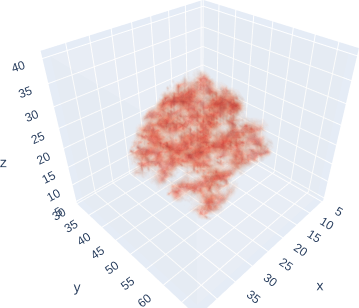
\includegraphics[height=6cm,width=\textwidth,keepaspectratio]{res_grid_comp.png}
        \caption{In the complex coordinate system.}
        \label{fig:res_grid_comp}
    \end{subfigure}%
    \begin{subfigure}{.5\textwidth}
        \centering
        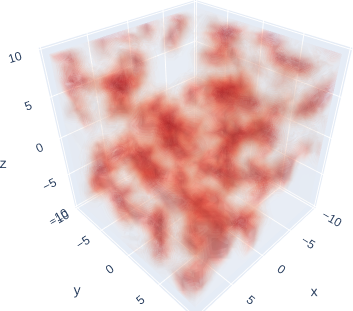
\includegraphics[height=6cm,width=\textwidth,keepaspectratio]{res_grid_res.png}
        \caption{In the local residue coordinate system.}
        \label{fig:res_grid_res}
    \end{subfigure}
    \caption{An amino acid residue represented as a voxel grid. The densities of all atom types are summed up to ease visualization.}
    \label{fig:residue_grid}
\end{figure}
Wrapping up, a protein's residue is represented by a $24 \times 24 \times 24 \times 207$ array of densities, as illustrated in \textbf{Figure \ref{fig:residue_grid}}. Projecting to the local residue coordinate system from the complex one is done with: $coord^{residue} = (coord^{complex} - origin^{residue}) \boldsymbol{\cdot} axis^{residue}$, and back to the complex one as: $coord^{complex} = coord^{residue} \boldsymbol{\cdot} (axis^{residue})^{-1} + origin^{residue}$.

\subsubsection{To that of the full complex one}

From the individual representations of a protein's residues, I reconstructed the full complex voxel grid using an Axis-Align Bounding Box (AABB). An AABB is constructed by extending the bounds of a box while adding to it new axis-aligned boxes. \textbf{Figure \ref{fig:aabb}} below illustrates the concept with a simple example of one bounding box created from two other boxes.
\begin{figure}[H]
    \centering
    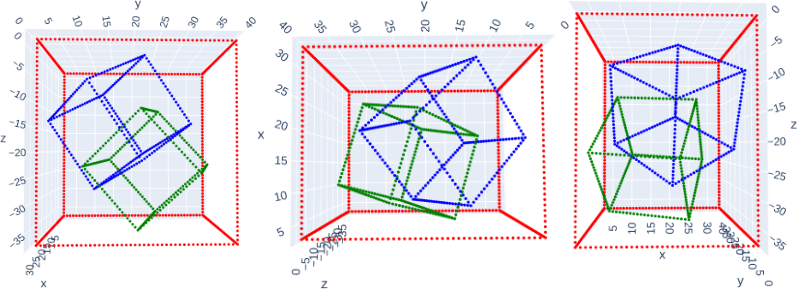
\includegraphics[height=6cm,width=\textwidth,keepaspectratio]{aabb.png}
    \caption{Three different views over the red AABB corresponding to the green and blue boxes.}
    \label{fig:aabb}
\end{figure}
In our case, the full complex grid corresponds to the red box, filled with all its residues' grids. As in the example above, residues' grids can overlap. \\
\textbf{Figure \ref{fig:complex_grid}} allows to visualize the density grid corresponding to a full complex. As one can see, some atoms do not contribute to the densities as they are too far from any residue's origin.
\begin{figure}[H]
    \centering
    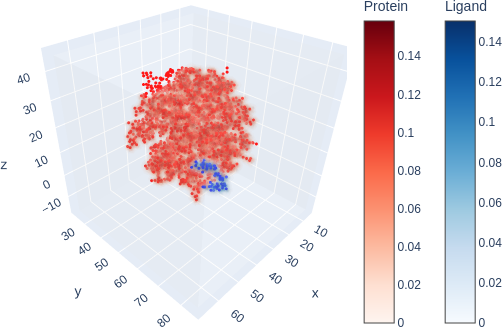
\includegraphics[height=6cm,width=\textwidth,keepaspectratio]{complex_grid.png}
    \caption{A complex represented as a voxel grid. In red the protein and in blue the ligand densities. The points correspond to the initial atoms' locations.}
    \label{fig:complex_grid}
\end{figure}

\subsubsection{The input, the output and the mask}
\label{sec:input_output_mask}

In the context of 2D image inpainting, it is very easy to define the input, the output and the mask: the corrupted image is the input, the reconstructed one is the output and the regions identified as corrupted compose the mask. To us, the definition of the input and the output is also fairly straightforward: the input is the density grid with only the protein's atoms contributions (red part of \textbf{Figure \ref{fig:complex_grid}}) and the output is the same density grid but with only the ligand's atoms contributions (blue part of the \textbf{Figure \ref{fig:complex_grid}}). \\

Defining the mask also seems quite simple: it is the ligand's region. But this formulation raises two issues: firstly, we are not supposed to know in advance the ligand's atoms' position ; secondly, we need to determine the region given some atoms' location. \\
Rather than using the ligand's region, we can use the complement (as in set theory) of the protein's region because we know that it should include the ligand's region. A chemical bond between a protein's and a ligand's atom is strictly longer than $2 \angstrom$, meaning that a ligand's atom cannot be closer to a protein's atom than $2 \angstrom$. Therefore, the protein's region can be defined as the voxels whose distance between its center and any protein's atom is smaller or equal than $2 \angstrom$. Taking the complement of this set as we suggested will result in the mask pointlessly large because we also know that ligand's atoms cannot be too far from the protein's ones. I added an additional constraint to exclude from the mask voxels at more than $3*2\angstrom$:
$$
\begin{array}{ll}
    too\_close = \{voxel \mid (\exists\: atom \in protein \mid \Vert voxel - atom \Vert\ \leq 2\angstrom)\} \\
    too\_far = \overline{\{voxel \mid (\exists\: atom \in protein \mid \Vert voxel - atom \Vert\ \leq 3*2\angstrom)\}} \\
    mask = too\_close \cup too\_far
\end{array}
$$
\textbf{Figure \ref{fig:mask}} illustrates the construction around a single protein's atom in 2D.
\begin{figure}[H]
    \centering
    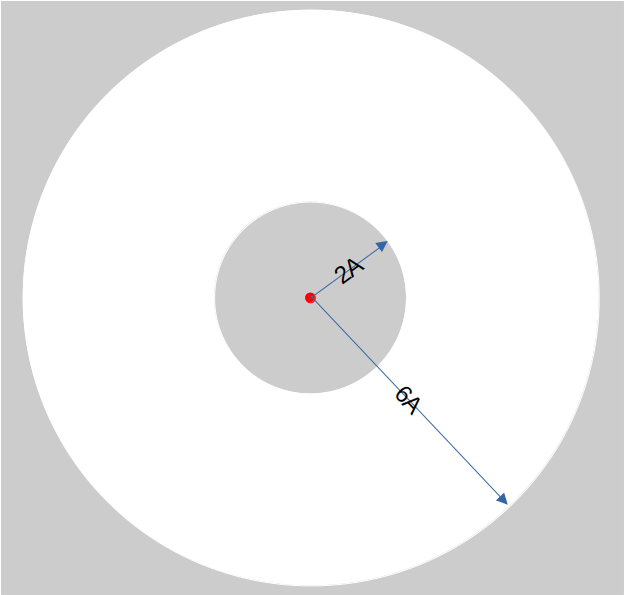
\includegraphics[height=3cm,width=\textwidth,keepaspectratio]{mask.png}
    \caption{In grey, the masked region for a single protein's atom (the red bullet), in 2D.}
    \label{fig:mask}
\end{figure}

\subsection{Generating the ligand through a CNN}

I will start with a short explanation of neural networks' functioning and the particularities of \textit{Convolutional} Neural Networks. Those prerequisites are necessary to understand the key concepts of DSNet \cite{DSNet} and the extensions I implemented for ligand generation.

\subsubsection{Introduction to (Convolutional) Neural Networks}
\label{sec:cnn}

In supervised learning, we want to find the function $f$ from our input space $X$ to our output space $Y$ that minimises the empirical risk:
$$R_{emp}(f) = \frac{1}{N}\sum_{i=1}^N L(f(x_i), y_i)$$
where $x_i$ and $y_i$ are available input (usually vectors) and output (vectors, scalars or categories) data, and $L$ is the loss function characterising the error between $f(x_i)$ and $y_i$. Finding such a function is NP-hard, therefore $f$ is often constrained to a particular family of functions (polynomial, exponential, etc...). Neural networks can be seen as another family of functions.

\paragraph{General functioning}
A neural network is made of several layers, stacked one after the other. We can express the function $f^{NN}$ of a neural network with $K$ layers as:
$$f^{NN} = f^K \circ f^{K-1} \circ ... \circ f^1$$
with $f^k$ being the function representing the $k^{th}$ layer. The size of the $k^{th}$ layer defines the codomain's dimension of $f^k$ and the domain's dimension of $f^{k+1}$. \\
Dense layers are the simplest kind of layer to think of, as they apply a linear transformation to their input. In matrix notation, it gives for layer $k$:
$$f^k(x) = \sigma_k(W_kx+b_k)$$
where $x$ in the normalized layer input vector, $W_k$ the weights matrix, $b_k$ the vector of bias and $\sigma_k$ the activation function. Activation functions play an important role in neural networks' architectures because they are making the function $f^{NN}$ non-linear, thus allowing the network to model non-linear problems. \\
A neural network learns from the data by updating its layers' weights in order to minimize the loss function $L$. Given the complexity of neural networks, finding a local minimum of $L$ is performed using \textit{Gradient Descent} (and its variations as Batch GD, MiniBatch GD, Stochastic GD, Momentum GD, Adaptive Momentum GD, Nesterov accelerated gradient, etc...). Intuitively, it corresponds to iteratively decreasing $L$ in the fastest possible way by updating the network's weights in the opposite direction of the gradient of $L$ given their current value. Formally, updating the weights after the $n^{th}$ iteration is done with:
$$W_{n+1} = W_n - \gamma * \nabla L(f^{NN}_n(x), y)$$
where $f^{NN}_n$ depends on $W_n$ and $\gamma$ is the learning rate, allowing the weights to change more or less rapidly. The choice of the learning rate is important, since a too small rate will slow down the convergence to a local minimum and a too large one might prevent the network from converging.

\paragraph{Convolution} CNN follow this general functioning, except for the fact that they are not mostly composed with dense layers but with \textit{convolutional} layers. A convolutional layer can represent more effectively features formed by adjacent pieces of information. Adjacent pieces of information might be neighboring pixels or words in Computer Vision or NLP. \\
In dense layers, every element of the output is weighted by every element in the input, whereas in a convolutional layer, the input's patches are multiplied with a learnable \textit{filter} (or \textit{kernel}) to generate the \textit{activation map} (or \textit{feature channel}). The filter is strided along every dimension of the input in order to process it completely. A convolutional layer might have several independent filters (meaning that they all have their own learnable weights) in order to capture different features. \\
In order to reduce dimensionality and enhance the expressivity of layers' nodes, a convolution is often followed by a pooling operation. The most common pooling is the \textit{max pooling}, extracting the maximum from activation maps' patches. Sometimes \textit{average pooling} is also used, while not as useful to improve expressivity it has the advantage of being an inversible operation. \\
In case of several filters, all the maps are finally stacked together to form the layer's output. The complete reasoning behind convolutional layers is illustrated in \textbf{Figure \ref{fig:conv_layer}}.
\begin{figure}[H]
    \centering
    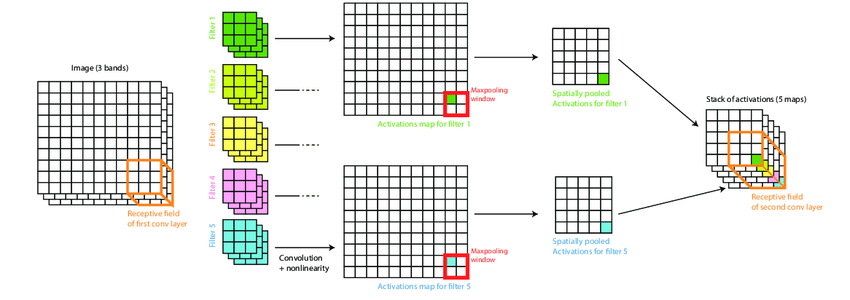
\includegraphics[height=6cm,width=\textwidth,keepaspectratio]{conv_layer.png}
    \caption{Schematisation of a convolutional layer applied to an image, from \cite{conv_layer_img}.}
    \label{fig:conv_layer}
\end{figure}
By stacking several convolutional layers, a network might learn features between elements more and more distant as features of previous features. They have been very useful in developing neural networks for Computer Vision, and in particular for image inpainting.

\subsubsection{2D image inpainting with DSNet}

DSNet \cite{DSNet} is a 2D image inpainting architecture introduced by Wang \textit{et al}. Like most inpainting networks, it follows the U-Net \cite{U_Net} architecture. U-Net networks have two convolutional branches, one traditional encoding branch where convolutional layers, as described in the previous paragraph, are stacked, and a decoding branch where pooling operations are replaced with upsampling operations. At each step in the encoding branch, the number of feature channels is doubled, and it is repeatedly halved in the decoding one. This allows to encode and decode the input in a non-linear way and to efficiently process high-resolution images while bypassing GPU memory limitations. \\
\begin{figure}[H]
    \centering
    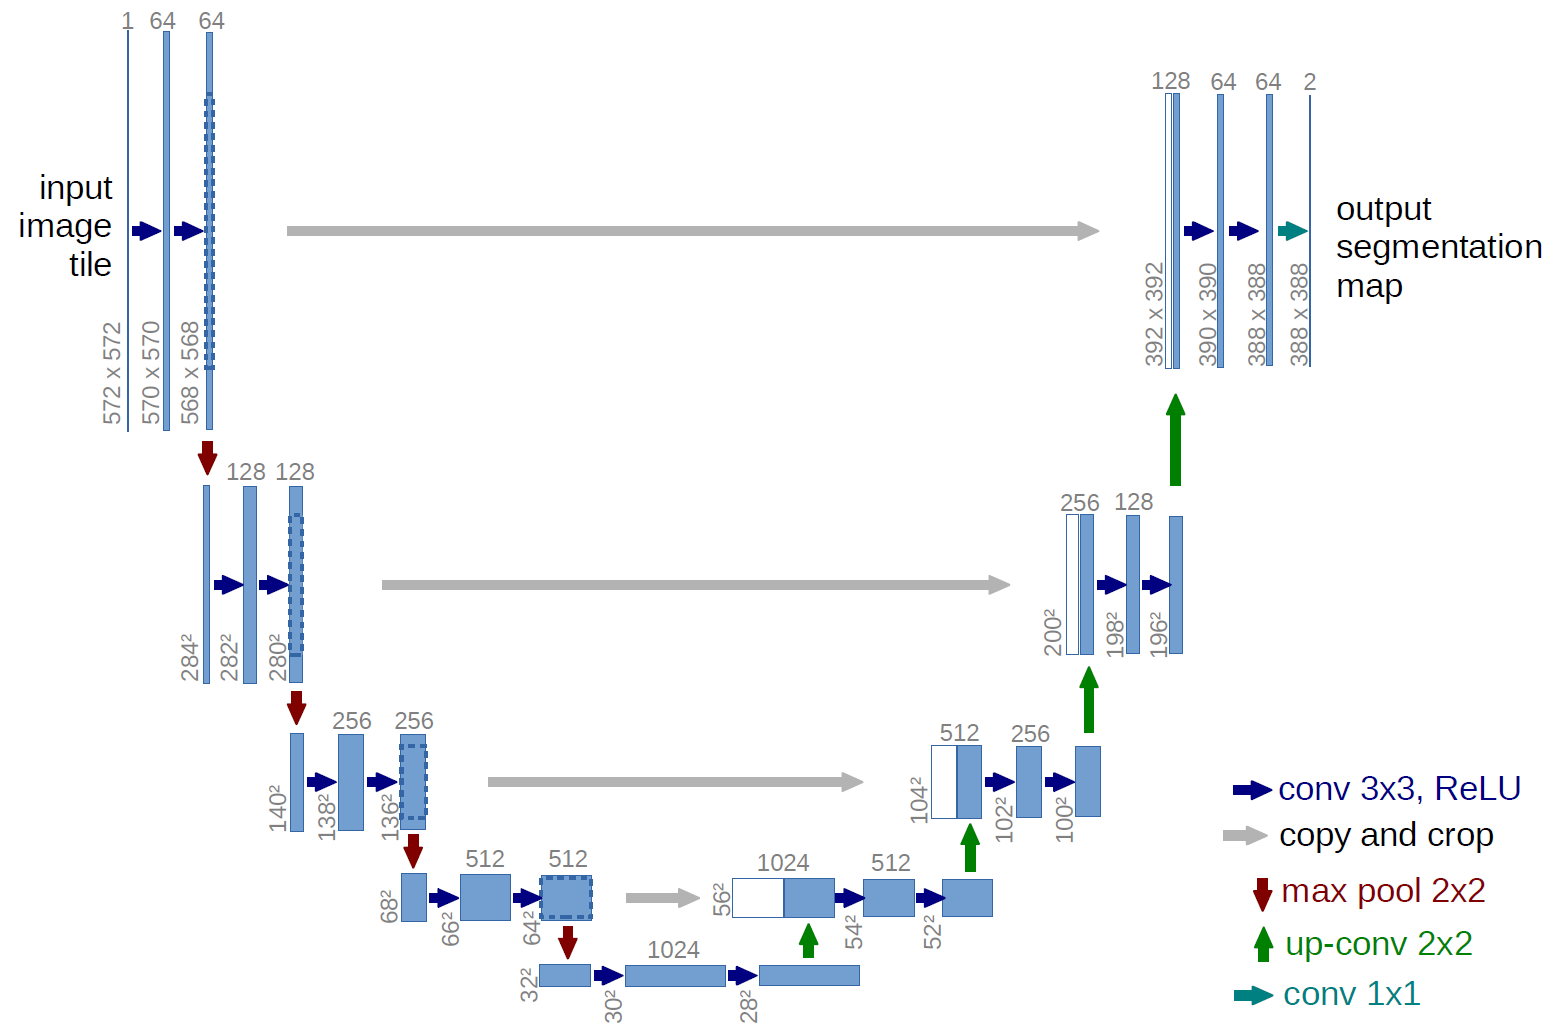
\includegraphics[height=6cm,width=\textwidth,keepaspectratio]{u_net.png}
    \caption{Overview of the U-Net architecture, from \cite{U_Net}.}
    \label{fig:u_net}
\end{figure}

DSNet introduces two key modules: the Validness Migratable Convolution (VMC) and the Regional Composite Normalization (RCN). \\
VMC allows the convolution to use more valid information when doing inpainting than traditional convolutional layers, by replacing masked pixels' values with valid pixels' values in the neighborhood. \textbf{Figure \ref{fig:dsnet_vmc}} illustrates it with a simple example.
\begin{figure}[H]
    \centering
    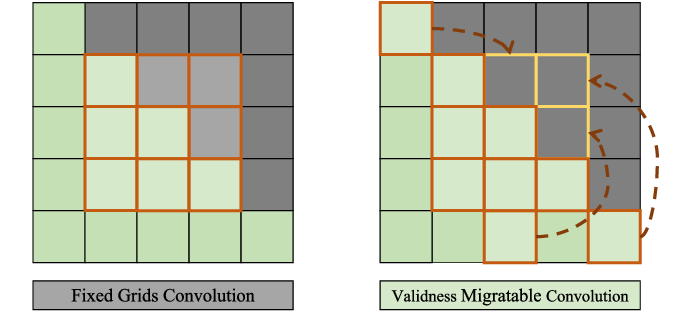
\includegraphics[height=3cm,width=\textwidth,keepaspectratio]{dsnet_vmc.png}
    \caption{Validness Migratable Convolution from \cite{DSNet}. In green the valid pixels are represented, and in grey the mask ones. The orange/yellow grid corresponds to the selected patch.}
    \label{fig:dsnet_vmc}
\end{figure}
In \hyperref[sec:cnn]{[\S3.3.1]}, I quickly mentioned that layer's inputs are normalized. Even though the reason behind it remains under discussion \cite{bn_ics,bn_smooth,bn_acc}, this normalization has been recognised to ease and accelerate neural network's convergence. With CNN it can be done in different ways: across a batch of inputs, along channels or groups of channels. RCN combines those three approaches and decouples them for masked and valid regions. \\
DSNet also reused the pixel-wise attention module proposed by \cite{pw_att}. The attention mechanism allows to learn features not only in the neighborhood but also from the background by identifying similar regions. Specifically, pixel-wise attention gives the network the ability to use features from the valid region's background to inpaint the masked one. \\

In order to numerically assess the quality of the inpainting and optimize the network's weights, DSNet uses a combination of five losses. \textit{Perceptual} and \textit{style} losses are commonly used in Computer Vision and evaluate the quality of the extracted features. They are computed using a separate pretrained network. The \textit{total variation} loss penalizes important variations between adjacent pixels. Finally, \textit{hole} and \textit{valid} losses measure the difference in the masked and valid regions between the ground truth and the prediction. \\
By dynamically utilizing information, DSNet got very good results, both qualitatively as shown in \textbf{Figure \ref{fig:2d_im_inp}}, and quantitatively by outperforming standard inpainting architectures on commonly used Computer Vision test datasets.

\subsubsection{Our extension for ligand generation}
\label{sec:ext}

Several stages were necessary before being able to generate a ligand given a protein using a network initially designed for 2D image inpainting. The architectures described here are the result of numerous trials and errors, but for the sake of clarity I have chosen to present only the main variations at the time of writing.

\paragraph{3 Dimensions}
The first step was to make DSNet usable with 3D images. This was relatively easy and fast, since most PyTorch built in 2D functions or classes employed in the DSNet architecture have their 3D equivalent. However, I also had to adapt some custom functions implementing the MVC, RCN and pixel-wise attention modules.

To validate this first stage, I used the MNIST database of handwritten digits \cite{mnist}. As the name suggests, this dataset is made of grey-scale images of handwritten digits. Those images are in 2D so I added a third dimension by stacking the original image with itself twice along the new dimension. I cropped them to the chosen resolution of the residues' grid voxel. In order to both replace the white color, as it is the "color" of the mask, and use inputs with three color channels, I concatenated the color channel with a $1\times2$ vector of zeros. Therefore, the resulting arrays were of size $24\times24\times24\times3$. The mask was randomly generated in the initial 2D space and going all the way through the third dimension. \\
Since the resulting 3D images were of a much lower resolution than the 2D images feeding DSNet I had to reduce the depth of the U-Net architecture. From initially eight encoding layers and eight decoding layers, I went down to four layers in each branch. \\
Finally, I removed the \textit{perceptual} and \textit{
style} losses, as the pretrained model they rely on is specific to 2D images. I also replaced the Mean Absolute Error (MAE) with Mean Square Error (MSE) in the other three losses. \\
\phantom{\quad} Having a working reconstruction, I moved to the second stage.

\paragraph{Independent residues as inputs}
In the 3D scenario, inputs and outputs were both $24 \times 24 \times 24 \times 1$ arrays. When using residues, the first change comes with the different sizes of the inputs and the outputs. As I mentioned in \hyperref[sec:input_output_mask]{[\S3.2.3]}, the generator's inputs are the protein's atoms density grids, and there are 167 different protein atom types, giving $24 \times 24 \times 24 \times 167$ arrays as inputs. On the other hand, its outputs are ligand atom density grids, with 40 different atom types, hence $24 \times 24 \times 24 \times 40$ arrays as outputs. In order to accommodate those sizes, the convolutional layers were updated to their final form, as displayed in \textbf{Table \ref{table:arch}}.
\begin{table}[H]
\centering
\caption{Ligand generator architecture.}
\resizebox{\textwidth}{!}{\begin{tabular}{ccccccccccc}
\hline
Layer & Input                 & Operator  & Normalization & In\_Size & Out\_Size & K\_size & S & P & C   & Activation \\
\hline
Enc1  & Res, Mask             & Conv      &               & 24       & 18        & 7       & 1 & 0 & 64  & ReLU       \\
Enc2  & F\_Enc1               & VMC       & RCN           & 18       & 12        & 7       & 1 & 0 & 128 & ReLU       \\
Enc3  & F\_Enc2               & VMC       & RCN           & 12       & 12        & 7       & 1 & 0 & 256 & ReLU       \\
Enc4  & F\_Enc3               & VMC       & RCN           & 6        & 3         & 3       & 2 & 1 & 512 & ReLU       \\
Dec5  & cat(F\_Enc3, F\_Enc4) & VMC       & RCN           & 3        & 6         & 3       & 1 & 1 & 256 & LeakyReLU  \\
Dec6  & cat(F\_Dec5, F\_Enc2) & VMC       & RCN           & 6        & 12        & 3       & 1 & 1 & 128 & LeakyReLU  \\
Att   & F\_Dec6               & Attention &               & 12       & 12        &         &   &   & 128 &            \\
Dec7  & cat(F\_Att, F\_Enc1)  & VMC       & RCN           & 12       & 18        & 3       & 1 & 1 & 64  & LeakyReLU  \\
Dec8  & cat(F\_Dec7, F\_In)   & Conv      &               & 18       & 24        & 3       & 1 & 1 & 40  & ReLU       \\
\hline
\end{tabular}}
\label{table:arch}
\end{table}
\textit{ReLU} has become the most popular activation function for helping neural networks to converge faster. However, since it clips negative values to zero, it can introduce a lot of null values in the layers' outputs which impact the network performance. This can be avoided using \textit{LeakyReLU}, where negative values are allowed to remain negative with a small slope, as visible in \textbf{Figure \ref{fig:l_relu}}.
\begin{figure}[H]
    \centering
    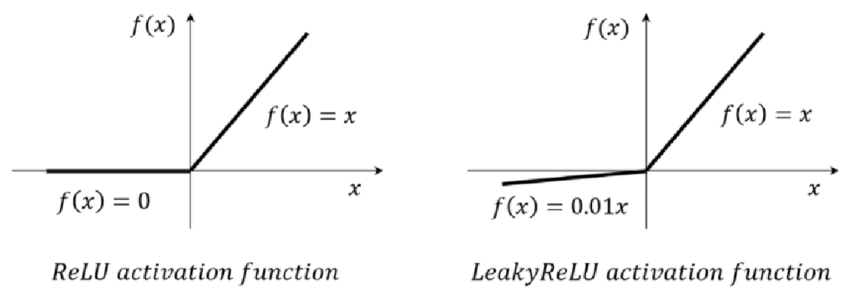
\includegraphics[height=3cm,width=\textwidth,keepaspectratio]{l_relu.png}
    \caption{ReLU and LeakyReLU activation functions.}
    \label{fig:l_relu}
\end{figure}
The second change concerns the loss function. In the following equations, $\rho_{x,y,z,k}$ refers to the density value of atom type $k$ in the voxel at location $(x,y,z)$ ; $\rho^{nonmask\_pred}$, $\rho^{mask\_gt}$, $\rho^{mask\_pred}$ refer respectively to generated densities in the non-masked space, ground truth and predicted densities in the masked space ; $K$ denotes the number of atom types ; $N^{nonmask}$ indicates the number of the non masked voxels and $N^{mask}$ the number of masked ones. \\
I kept the \textit{total variation} ($L^{tv}$) loss:
$$
\begin{array}{l@{}l}
    L^{tv} = \frac{1}{N^{mask}*K} \sum_{x,y,z,k}
    &{} (\rho_{x,y,z,k}^{mask\_pred} - \rho_{x+1,y,z,k}^{mask\_pred})^2 + \\
    &{} (\rho_{x,y,z,k}^{mask\_pred} - \rho_{x,y+1,z,k}^{mask\_pred})^2 + \\
    &{} (\rho_{x,y,z,k}^{mask\_pred} - \rho_{x,y,z+1,k}^{mask\_pred})^2
\end{array}
$$
and the \textit{hole} ($L^{ligand}$) loss:
$$
L^{ligand} = \frac{1}{N^{mask}*K} \sum_{x,y,z,k} (\rho_{x,y,z,k}^{mask\_gt} - \rho_{x,y,z,k}^{mask\_pred})^2
$$
But, I updated the \textit{valid} loss ($L^{protein}$) since the ligand generation should only happen in the masked region, while the non-masked region, identified as not able to hold ligand atoms, should be empty. Meaning that densities in the non-masked region should be null.
$$
L^{protein} = \frac{1}{N^{nonmask}*K} \sum_{x,y,z,k} (\rho_{x,y,z,k}^{nonmask\_pred})^2
$$
And, I added a \textit{penalization} term ($L^{steric}$) responsible for penalizing the number of non-null densities. In the same spirit as $L_1$ regularization added to Lasso, it is not desirable to have several non-null densities in the same voxel as a voxel can only contain at most one atom.
$$
L^{steric} = \frac{1}{N^{mask}} \sum_{x,y,z} \frac{1}{K} \sum_{k} \vert \rho_{x,y,z,k}^{mask\_pred} \vert
$$
The losses are weighted in order to give more importance to the term $L^{ligand}$ that should hold most of the predicting power.
$$
L^{total} = w^{ligand} * L^{ligand} + w^{protein} * L^{protein} + w^{tv} * L^{tv} + w^{steric} * L^{steric}
$$
Quite quickly, the results were extremely promising so we decided to further extend the architecture.

\paragraph{Learning on the complexes}
In the previous paragraph, the network was fed with residues and the loss was computed using the residues as if they were independent and not part of a larger complex. We wanted instead to consider the residues as part of a complex. Feeding the network directly with full complexes would have been ideal, but given our architecture's type, it was almost impossible. Firstly, the size of the complexes' AABB is much larger than the fixed size of the box placed around residues, resulting in some additional computational costs and, more importantly, memory overhead. Secondly, complexes have different sizes, which would result in different input sizes and the need to either up-sample or down-sample them before processing. Finally, the network may loose the invariance property introduced by using orientated grid around residues. \\

While still feeding the network with residues, the generated residue densities are projected back from the local coordinate system to the complex coordinate system. Since residues' grids can overlap, the complex's densities are computed by making the weighted average of its residues' densities.
$$
\rho_{x,y,z,k}^{complex} = \frac{1}{N_{x,y,z}^{residue}} \sum_{i=1}^{N_{x,y,z}^{residue}} w_{x,y,z,i} * \rho_{x,y,z,k,i}^{residue}
$$
We consider that generated residues' densities are more reliable when closer to the residues' origin. Therefore, in order to give more importance to the most reliable densities, the inverse of the distance between the voxels' centers and the residue's origin ($+1$ to avoid dividing by zero at the origin's voxel) is used as the weight.
$$
w_{x,y,z,i} = \frac{1}{1+||center_{x,y,z}^{voxel} - origin_{x,y,z,i}^{residue}||_2}
$$
After having processed all the protein's residues, the loss is computed as previously, but with the complex densities. Finally, the network internal weights are updated according to this global loss, using Stochastic Gradient Descent, as gradients are not computed after having evaluated a mini-batch of residues but after the evaluation of a single complex. \\
\textbf{Figure \ref{fig:arch}} presents a simplified overview of the full architecture.
\begin{figure}[H]
    \centering
    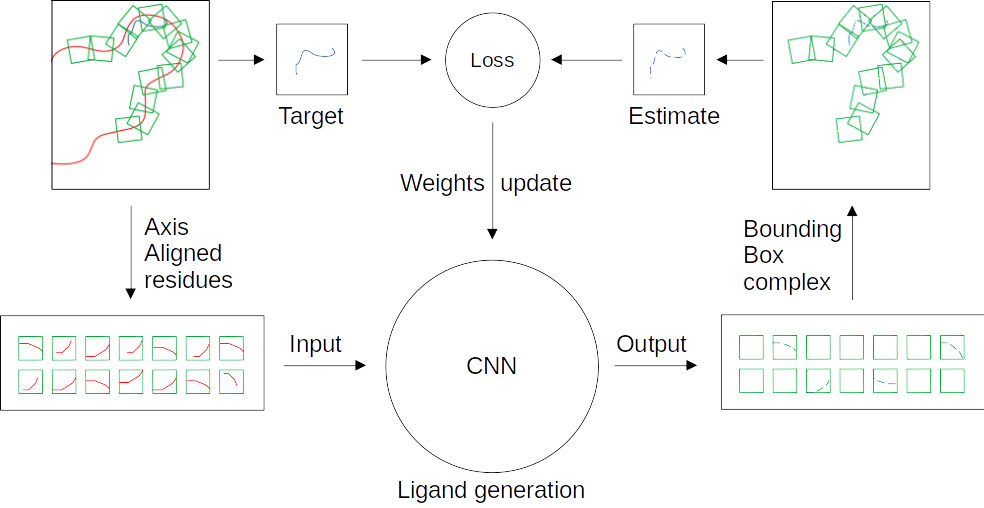
\includegraphics[height=6cm,width=\textwidth,keepaspectratio]{arch.png}
    \caption{Graphical representation of the proposed architecture. The protein is in red and the ligand in blue. The green boxes represent the amino acid residues.}
    \label{fig:arch}
\end{figure}

\paragraph{End-to-end}

The ultimate goal for ligand generation is to output the coordinates or the locations of the ligand in an end-to-end fashion. Meaning that no additional post-processing is necessary on the neural network's output. \\

I had very little time to attempt this, so I tried quite a straightforward approach, that is pixel-wise classification. Instead of outputting a density grid, the network could directly output a probability grid for the presence of an atom with a certain type in every voxel. I added an additional filter to the last convolutional layer (last line of \textbf{Table \ref{table:arch}}) to allow a category corresponding to "no ligand atom" and I replaced the ReLU activation with a Softmax.
$$
Softmax(\rho_{x,y,z,k}) = \frac{exp(\rho_{x,y,z,k})}{\sum_i exp(\rho_{x,y,z,i})}
$$
Softmax is a standard choice for multiple classes classification, since its outputs lie in the range $[0,1]$ and summed up to $1$. \\
Finally, I had to adapt the loss function to a classification task. I only used the negative log likelihood loss, without further regularization terms.
$$
L^{nll} = \frac{1}{\sum_{x,y,z} w_{(v_{x,y,z})}}\sum_{x,y,z} -w_{(v_{x,y,z})}log(\hat{v}_{x,y,z,(v_{x,y,z})})
$$
where, $w_{(v_{x,y,z})}$ is the weight associated with the category of $v_{x,y,z}$ and $\hat{v}_{x,y,z,(v_{x,y,z})}$ means that only predicted probabilities for the correct category are taken into consideration. I assigned all the weights to $1$, except for the one corresponding to the category "no ligand atom" that is equal to the inverse of the number of voxels to prevent the neural network from always predicting that category as it is over-represented compared to the others.

\clearpage

\section{Results}

Beforehand, I would like to mention that all the implementation of the work described in the previous section has been realized in Python \cite{Python}, heavily using NumPy \cite{NumPy} and  PyTorch \cite{PyTorch} libraries, plus others cited along the way. The figures of the report itself have mostly been created using Plotly \cite{Plotly}. \\
My implementation of the different architectures we tried and the pre-processing on the data is hosted on GRICAD GitLab plateform. I put efforts into tracking our numerous implementation attempts by using several Git branches. I also did my best to write, organise and comment my code such that it is understandable and easy to re-use by others. \\
Finally, training of the networks was performed using their GPU cluster. \url{https://gricad.univ-grenoble-alpes.fr/} \\

\subsection{3D MNIST}

As mentioned in \hyperref[sec:ext]{[\S3.3.3]}, the aim of the experiment on the 3D MNIST dataset was only to validate the 3D extension of the DSNet architecture. Therefore, I did not train the network for a very long time, and as the loss, visible in \textbf{Figure \ref{fig:3d_mnist_loss}}, was still decreasing when training ended, it seems that the network could have continued to learn. I used a batch size of 12 images, with a training set of 42000 images and a test set of 28000 images.
\begin{figure}[H]
    \centering
    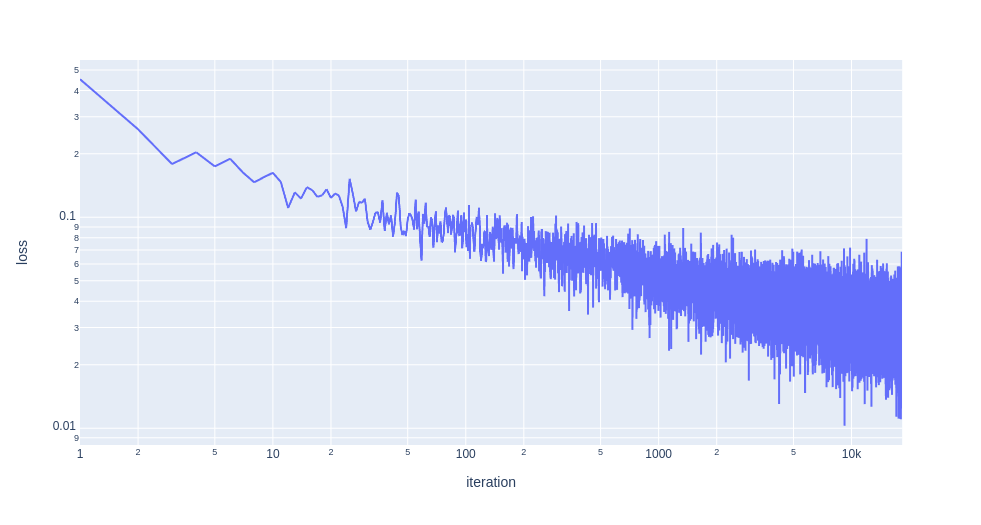
\includegraphics[height=6cm,width=\textwidth,keepaspectratio]{3d_mnist_loss.png}
    \caption{Evolution of the total loss function during training in log-log scale.}
    \label{fig:3d_mnist_loss}
\end{figure}
Given the objective of this experiment, I did not validate the results of the full test set, but only on a small part of it. Despite the early termination of the training, the obtained reconstruction was already really good, as shown by the examples in \textbf{Figure \ref{fig:3d_mnist_imp}}.
\begin{figure}[H]
    \centering
    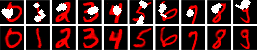
\includegraphics[height=3cm,width=\textwidth,keepaspectratio]{3d_mnist_imp.png}
    \caption{Reconstruction examples on the 3D MNIST dataset. Pixels values are averaged on the third dimension to ease 2D visualization.}
    \label{fig:3d_mnist_imp}
\end{figure}

\subsection{PDBbind}

In order to test the capabilities of our network to generate a probable ligand given a real protein, we used the PDBbind dataset, randomly splitted into a training and a test set, as described in \hyperref[sec:dataset]{[\S3.1.1]}.

\subsubsection{On the "hyper over-fitting" road}
First I tried to generate the ligand at the residue level. For this, I used a batch size of 30 residues. Qualitative overviews of the reconstructed ligand, like the one in \textbf{Figure \ref{fig:gen_res_wrong}}, were very impressive.
\begin{figure}[H]
    \centering
    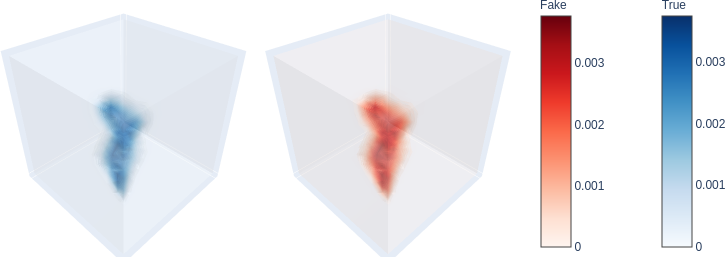
\includegraphics[height=4cm,width=\textwidth,keepaspectratio]{gen_res_wrong.png}
    \caption{Averaged densities of true (blue) and generated (red) ligands.}
    \label{fig:gen_res_wrong}
\end{figure}
Therefore, we pressed onto the generation on the full complex. The first predicted ligand was, once again, visually perfectly similar to the ground truth one. However, I realized that all the generated complexes' representations were strictly identical. The issue came from the plain text files I used to generate the HDF5 file (see \hyperref[sec:pdbbind]{[\S3.1]}). They were all the same, meaning that I was both training and testing with a single protein-ligand complex. I did not realize it earlier because I was visualizing the 3D representation of the proteins using PyMOL and valid PDB files, and when working with the residues I was seeing different amino acid residues, without suspecting that they were belonging to only one protein.

\subsubsection{And back to reality}
\label{sec:res-reality}
After this wandering and having retrieved the correct files, I trained the network again. On one hand, the evolution of the total loss, in \textbf{Figure \ref{fig:loss_complex-all}}, looks good since it quickly tends toward zero. On the other hand, such a slope on a log-log plot might seem suspicious given the apparent complexity of the task.
\begin{figure}[H]
    \centering
    \begin{subfigure}{.5\textwidth}
        \centering
        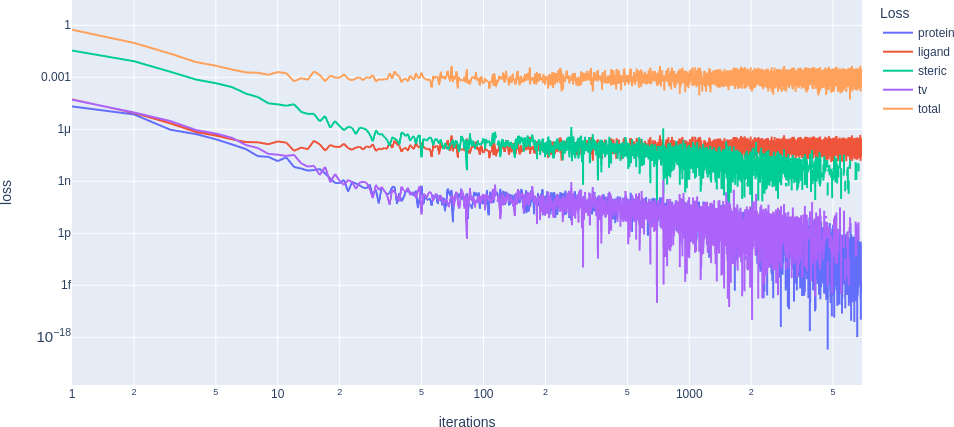
\includegraphics[height=6cm,width=\textwidth,keepaspectratio]{loss_complex-all.png}
        \caption{All the losses.}
        \label{fig:loss_complex-all}
    \end{subfigure}%
    \begin{subfigure}{.5\textwidth}
        \centering
        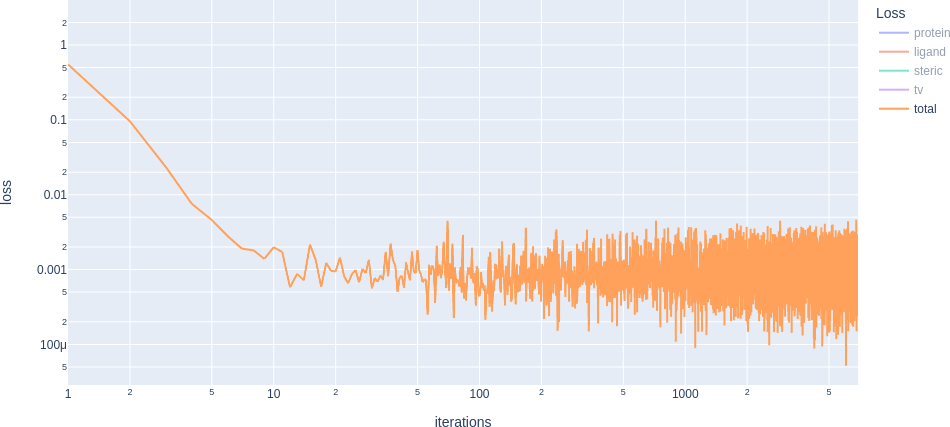
\includegraphics[height=6cm,width=\textwidth,keepaspectratio]{loss_complex.png}
        \caption{The total loss.}
        \label{fig:loss_complex-tot}
    \end{subfigure}
    \caption{Log-log evolution of the losses while training on the complexes.}
    \label{fig:loss_complex}
\end{figure}
Indeed, the results in \textbf{Figure \ref{fig:result_complex}} show that the network is not learning what we want and simply outputs zeros. By looking at the histogram it is not that surprising, since almost all the densities inside the masked region are equal to zero.
\begin{figure}[H]
    \centering
    \begin{subfigure}{.5\textwidth}
        \centering
        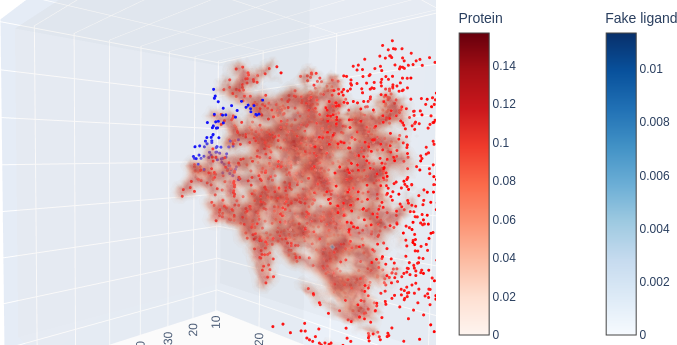
\includegraphics[height=6cm,width=\textwidth,keepaspectratio]{result_complex-quali.png}
        \caption{Ligand reconstruction. The points correspond to the ground truth location of the atoms. In blue, the ligand and in red, the protein.}
        \label{fig:result_complex-quali}
    \end{subfigure}%
    \begin{subfigure}{.5\textwidth}
        \centering
        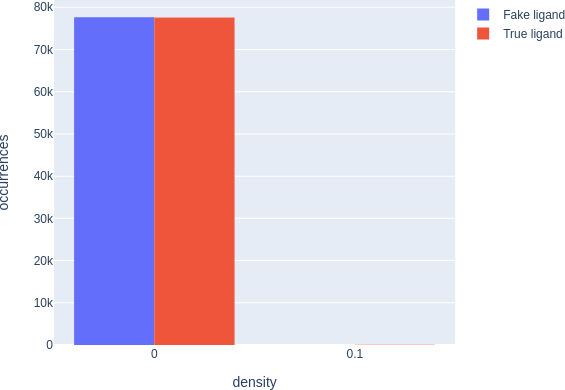
\includegraphics[height=6cm,width=\textwidth,keepaspectratio]{result_complex-hist.png}
        \caption{Histogram of the densities in the masked region.}
        \label{fig:result_complex-hist}
    \end{subfigure}
    \caption{Results of the generation on the full complex.}
    \label{fig:result_complex}
\end{figure}
This posed a new challenge and our first attempt to solve it was to train using a smaller mask, defined from the ligand instead of the protein, while still doing the generation using the large one (as described in \hyperref[sec:input_output_mask]{[\S3.2.3]}). Still,
the output were very small densities in the entire masked region. \\
We though that the issue might then be the range $[0,1]$ of our densities and the use of MSE losses. While MSE strongly penalizes larger errors when they are strictly greater than $1$, it is the contrary when they are strictly smaller than $1$. Therefore, we replaced it with the Binary Cross Entropy (BCE) when computing $L^{ligand}$. 
$$
L^{ligand\_bce} = \frac{1}{N^{mask}*K} \sum_{x,y,z,k} \rho_{x,y,z,k}^{mask\_gt} * log(\rho_{x,y,z,k}^{mask\_pred}) + (1-\rho_{x,y,z,k}^{mask\_gt}) * log(1-\rho_{x,y,z,k}^{mask\_pred})
$$
As exhibited in \textbf{Figure \ref{fig:loss_complex-bce}}, after a thousand iterations the optimization does not converge to a minimum which seems to indicate that the network is not outputting null densities anymore. But the monotony of the loss implies additional difficulties. \\
\begin{figure}[H]
    \centering
    \begin{subfigure}{.5\textwidth}
        \centering
        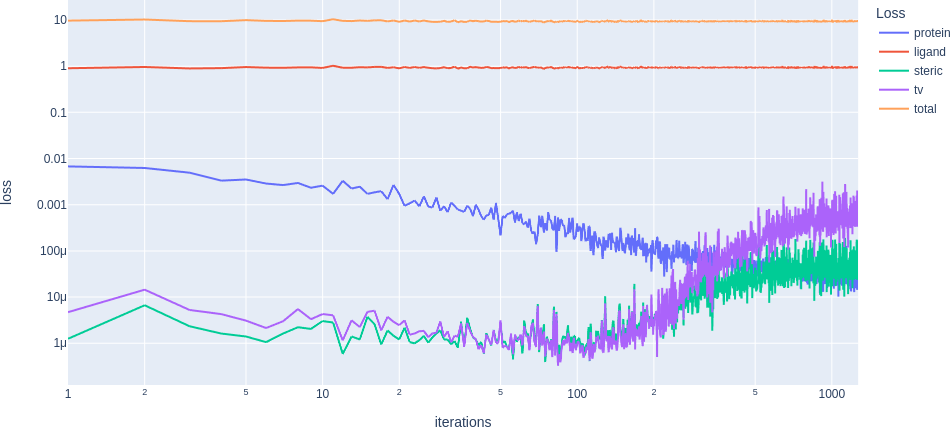
\includegraphics[height=6cm,width=\textwidth,keepaspectratio]{loss_complex-bce-all.png}
        \caption{All the losses, in log-log scale.}
        \label{fig:loss_complex-bce-all}
    \end{subfigure}%
    \begin{subfigure}{.5\textwidth}
        \centering
        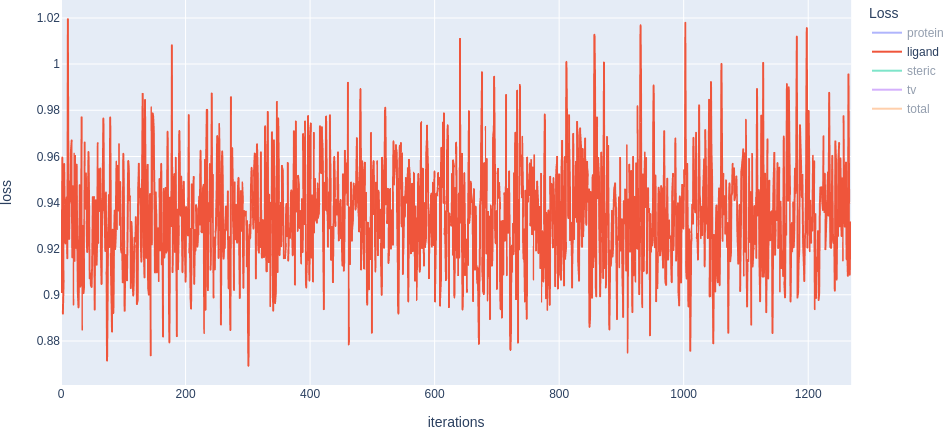
\includegraphics[height=6cm,width=\textwidth,keepaspectratio]{loss_complex-bce-lig.png}
        \caption{The ligand loss, $L^{ligand}$.}
        \label{fig:loss_complex-bce-lig}
    \end{subfigure}
    \caption{Evolution of the losses while training on the complexes using BCE in $L^{ligand}$.}
    \label{fig:loss_complex-bce}
\end{figure}
Thanks to the weights used in the negative log likelihood loss, the end-to-end approach should not suffer from the "dying densities" problem. Indeed, from the evolution of the loss, visible in \textbf{Figure \ref{fig:loss_end-to-end}}, it seems that the weights are playing their role. But it is also noticeable that, as in regression scenario using BCE, the network is not able to learn at all, given that the loss has not decreased after more than 5,000 iterations.
\begin{figure}[H]
    \centering
    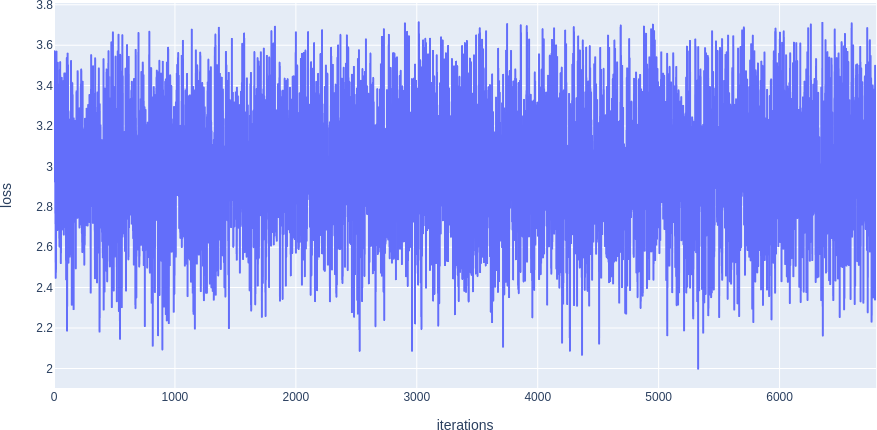
\includegraphics[height=8cm,width=\textwidth,keepaspectratio]{loss_end-to-end.png}
    \caption{Evolution of the negative log likelihood loss while training in the end-to-end fashion.}
    \label{fig:loss_end-to-end}
\end{figure}

The reality is much harder than the "hyper over-fitting" world and the network performances should be noticeably improved before justifying the use of the "hard" test set described in \hyperref[sec:hard]{[\S3.1.2]}.

\clearpage

\section{Outlook}

The over-fitting false lead has the merit of showing that on very simple and repetitive structures our architecture is able to learn something. Surely not the physics behind protein-ligand interactions, given the results encountered when working with complicated and diverse complexes. But with more adjustments, failures, and more readjustments, maybe we could hope to get closer. \\
It seems that our network struggles with the high dimensionality induced by our dense representation of the protein-ligand complex. To overcome this, there are a few leads we did not have time to investigate:
\begin{itemize}
    \item increasing the encoder/decoder depth. Most of the networks relying on the U-Net architecture use a depth of at least 8. Maybe using a depth larger than 4 could improve the learning capabilities of our network.
    \item increasing the number of convolutional filters in the encoding/decoding layers. Our first encoding layer reduces the number of channels from 167 atom types to 64 features. In classical U-Net architectures, the first layer increases it from 3 color channels to 64 features. In combination with the previous point, this could bring improvements, at the cost of a very high GPU memory use.
    \item inserting a linear encoding layer before the U-Net. Using a learnable linear transformation $Y = X \boldsymbol{\cdot} A + B$ before the convolutional part of the network would decrease the dimensionality and avoid the increased GPU memory use of the two previous points. We can think about this additional layer as a learnable Principal Component Analysis (PCA) by enforcing unit normalization on $A$ and introducing penalization terms to induced $A$ orthogonality and minimize the covariance of $Y$ features.
\end{itemize}
Another challenge for our network is the distribution of our data. Distinguishing between null values (where there is no ligand) and very small densities (where the ligand is) proved to be hard given our architecture. We saw that transforming the regression task into a classification one allowed to avoid this difficulty (while introducing other questions). Sticking to the regression approach, we started to investigate some ideas to seek for improvements:
\begin{itemize}
    \item using a smaller more precise mask during training, as mentioned in \hyperref[sec:res-reality]{[\S4.2.2]}.
    \item redefining the loss contributions, as explained in \hyperref[sec:res-reality]{[\S4.2.2]}.
    \item adjusting the range of our inputs. The atom densities lie in the range $[0,1]$, but most of the time the maximum bound of this range can be reduced below $0.1$. This could negatively impact the use of BCE, and more probably the learning of our network, even without BCE. Normalizing the densities such that their maximum bound is closer or equal to $1$ could be a factor of improvement.
\end{itemize}
I did not had time to propose a network taking into account the last four points, but it may allow some progress, and probably some more challenges as well! \\

As already mentioned in \hyperref[sec:pbstat]{[\S2.1.2]}, several other types of neural networks could have been extended for ligand generation. GAN and GNN intuitive functioning are quite different than the one behind image inpainting. On the contrary, recent 3D completion architectures based on sparse point cloud representation \cite{ProtRepr} (like cGCA \cite{cGCA} or PDR \cite{PDR}) could be highly interesting to address drug generation in an end-to-end fashion.

\clearpage

\printbibliography

\end{document}